
\documentclass[10pt]{article}
\usepackage{tmlr}

\usepackage{hyperref}
\usepackage{url}
\usepackage{booktabs}
\usepackage{multirow}
\usepackage{graphicx}
\usepackage{amsmath}
\usepackage{xcolor}
\usepackage{microtype}
\usepackage{float}
\usepackage{tikz}
\usetikzlibrary{arrows.meta, shapes.geometric, positioning, fit, backgrounds, calc, decorations.pathreplacing}
\usepackage{amssymb}
\usepackage{pifont}
\newcommand{\cmark}{\ding{51}}
\newcommand{\xmark}{\ding{55}}

% Suppress math_commands if not needed
% \input{math_commands.tex}

\title{Committed to the Hypothesis: LLM Agents as Stubborn Scientists\\
       in Neural Architecture Search}

% Authors hidden for blind review
\author{\name Anonymous Authors \email anonymous@anonymous.edu \\
      \addr Anonymous Institution}

\def\month{MM}
\def\year{YYYY}
\def\openreview{\url{https://openreview.net/forum?id=XXXX}}

\newcommand{\haas}{\textsc{HAAS}}
\newcommand{\nasbench}{NAS-Bench-201}
\newcommand{\cellstr}[1]{\texttt{\small #1}}

\begin{document}

\maketitle

\begin{abstract}
LLM-guided search suffers from consensus bias: agents that generate and refine
architectural proposals under critique converge prematurely toward well-established
designs, abandoning heterodox ideas at the first sign of resistance. We introduce
the \textbf{Heterodox Agent Architecture Search} (\haas{}) framework, which
addresses this by pre-committing an agent to a non-negotiable architectural
hypothesis. Rather than revising the hypothesis when challenged, the agent must
defend it and seek improvements that remain within the committed constraint ---
analogous to a stubborn scientist who explores the consequences of a minority
hypothesis rather than deferring to the prevailing consensus. We validate
\haas{} in two phases: a free-text behavioral study across seven architectural
hypotheses, and a controlled comparison on \nasbench{}/NATS-TSS where
compliance is exact and performance is pre-evaluated. Committed agents
maintain hypothesis fidelity throughout, while standard generate-refine
baselines collapse under the first challenge. In one case, the enforced
constraint leads \haas{} to \emph{outperform} the unconstrained baseline,
suggesting that directed commitment can expose favorable regions of the
search space that consensus-seeking agents avoid.
\end{abstract}

%-----------------------------------------------------------------------
\section{Introduction}
\label{sec:intro}
%-----------------------------------------------------------------------

The use of large language models (LLMs) as search agents in neural architecture
search (NAS) has produced a wave of recent systems that generate, evaluate, and
refine architectural proposals through natural language
\citep{zheng2023can,nasir2024llmatic}. A recurring design pattern is the
generate-critique-refine loop: an agent proposes an architecture, an evaluator
identifies weaknesses, and the agent revises its proposal accordingly. This loop
is intuitive and generally effective when the goal is to improve a proposal
toward consensus quality. Indeed, iterative agent loops are now producing
genuine scientific results beyond NAS: \citet{feng2026aletheia} report an
autonomous mathematics agent solving 6 of 10 previously unpublished research
problems, and \citet{karpathy2026autoresearch} demonstrates an agent
autonomously discovering improvements to an already-optimized neural network
training pipeline through hundreds of iterative code changes. In both cases,
the agent's ability to maintain a productive search direction across many steps
--- rather than collapsing to a safe default --- is central to the result.

In open-ended design tasks like NAS, however, this same loop is systematically
biased against heterodox ideas. When a critic challenges an architecture that
violates well-established design norms --- say, a cell with no skip connections,
or a block using only 1$\times$1 convolutions --- the path of least resistance
is capitulation. The agent has no incentive to hold
its ground; every revision that introduces skip connections, pooling, or 3$\times$3
convolutions is rewarded by a lower critique score, regardless of whether the
original constraint might have value in a specific regime.

We call this \textbf{consensus bias}: the tendency of LLM-guided search to
collapse toward the design consensus encoded in the model's pretraining
distribution, particularly under adversarial pressure. It is the machine
analogue of the social conformity problem that affects human scientists: the
pressure to adopt the accepted view of a field, even when an individual
scientist has specific reasons to believe the minority position.

The analogy suggests a remedy. In the history of science, fruitful heterodox
ideas have often been driven by \emph{committed} scientists who maintained their
hypotheses against social pressure long enough to accumulate the evidence needed
to evaluate them fairly. Darwin delayed publication of the theory of evolution
for twenty years; Semmelweis insisted on handwashing in the face of institutional
rejection; Marshall ingested \textit{H. pylori} to demonstrate the bacterial
theory of ulcers. The commitment was not epistemic irrationality --- it was a
deliberate strategy to avoid premature abandonment of an idea that the consensus
had not yet had time to evaluate.

We introduce the \textbf{Heterodox Agent Architecture Search} (\haas{})
framework, which operationalizes this commitment mechanism in an LLM agent loop.
A \haas{} agent is initialized with a non-negotiable architectural hypothesis
and instructed to \emph{steelman} --- present the strongest possible defense of
--- its commitment when challenged, rather than revise the hypothesis itself.
The agent is free to explore different instantiations of the hypothesis, but
the constraint encoded by the hypothesis is inviolable. The commitment is to
the \emph{constraint}, not to any specific architecture.

We make the following contributions:

\begin{enumerate}
  \item We identify and characterize \textbf{consensus bias} as a systematic
    failure mode of generate-critique-refine LLM search, with empirical evidence
    from seven architectural hypotheses in a free-text proposal setting (Phase~1).

  \item We introduce the \haas{} commitment mechanism and demonstrate that it
    maintains hypothesis fidelity throughout the search trajectory, with a
    qualitatively distinct failure mode (semantic drift rather than capitulation).

  \item We provide the first controlled comparison of committed vs.\ baseline
    agents on \nasbench{} \citep{dong2020nasbench201}, where constraint compliance
    is exact and performance is pre-evaluated, eliminating confounds from training.

  \item We show that constraint-enforced search can \emph{outperform}
    unconstrained search when the constraint aligns with a favorable subspace
    structure, and characterize the conditions under which this occurs.
\end{enumerate}

%-----------------------------------------------------------------------
\section{Related Work}
\label{sec:related}
%-----------------------------------------------------------------------

\paragraph{LLM-guided neural architecture search.}
Early NAS methods relied on reinforcement learning \citep{zoph2017neural} or
evolutionary algorithms \citep{real2019regularized} to search cell topologies.
Recent work has replaced the search controller with an LLM, exploiting its
knowledge of architectural design principles to generate more informed proposals.
\citet{zheng2023can} explore the feasibility of using GPT-4 as a black-box
optimizer for NAS; \citet{nasir2024llmatic} combine LLMs with quality-diversity
optimization on \nasbench{}. In all of these systems, the LLM acts as a proposal
generator implicitly biased toward the consensus design patterns encoded in
pretraining. \haas{} targets this bias directly.

\paragraph{Scientific discovery agents.}
Several recent systems cast LLMs as autonomous scientists. The AI Scientist
\citep{lu2024aiscientist} generates, evaluates, and publishes machine learning
research end-to-end. SciAgents \citep{ghafarollahi2024sciagents} uses a
multi-agent system to advance materials discovery through autonomous hypothesis
generation and refinement. \citet{feng2026aletheia} introduce Aletheia, an
autonomous mathematics research agent powered by Gemini~3 Deep Think that
solved 6 of 10 open problems from the First Proof benchmark
\citep{firstproof2026} --- a curated set of unpublished research-level
questions contributed by professional mathematicians --- through iterative
solution generation and formal verification. \citet{karpathy2026autoresearch}
reports an agent that autonomously optimizes a neural network training codebase
through iterative code modification and short training runs, discovering
genuine improvements on a pipeline that had been manually refined for years.
\citet{knuth2026claude} documents Claude~Opus~4.6 exploring 31 formulations
of a graph decomposition problem before arriving at a general solution that
surprised the problem's author. In each case the agent's value comes not from
a single inspired proposal but from sustained iterative exploration within a
problem structure. \haas{} studies what happens when that structure is made
explicit as a committed hypothesis: whether enforced direction improves or
constrains the quality of what is ultimately found.

\paragraph{Critique-and-refine agent loops.}
Constitutional AI \citep{bai2022constitutional} introduced the
critique-revision loop as a technique for aligning LLM output. ReAct
\citep{yao2023react} interleaves reasoning and action for decision-making tasks.
Chain-of-thought prompting \citep{wei2022chain} elicits step-by-step reasoning
that improves structured output quality. \haas{} builds on these foundations
but reframes the role of critique: rather than using it to steer the agent toward
the evaluator's preferred design, critique becomes a signal for the agent to
identify improvements within its committed hypothesis, without abandoning the
constraint itself.

\paragraph{NAS benchmarks.}
\nasbench{} \citep{dong2020nasbench201} defines a cell search space with 15,625
pre-evaluated architectures on CIFAR-10, CIFAR-100, and ImageNet-16-120, enabling
exact performance lookup without training. NATS-TSS \citep{dong2021nats} is the
topology search extension of the same benchmark. We use NATS-TSS CIFAR-10
accuracies as the ground truth performance signal throughout Phase~2, which
eliminates training variance from the comparison.

%-----------------------------------------------------------------------
\section{Method}
\label{sec:method}
%-----------------------------------------------------------------------

\subsection{Hypotheses}
\label{sec:hypotheses}

A \haas{} hypothesis is a natural language claim about which architectural
properties should or should not be present, together with an operationalization
of that claim as a constraint on the search space. Table~\ref{tab:hypotheses}
lists all seven hypotheses used in this study. Four of them (no\_skip,
sparse\_cell, pure\_conv, no\_3x3) have direct operationalizations in the
\nasbench{} cell format and were evaluated in both phases. The remaining three
(no\_attention, asymmetric\_depth, shared\_weights) apply to free-text
architectures evaluated only in Phase~1.

\begin{table}[t]
\caption{Architectural hypotheses evaluated in this study.}
\label{tab:hypotheses}
\begin{center}
\small
\begin{tabular}{llp{5.5cm}}
\toprule
\textbf{ID} & \textbf{Phase} & \textbf{Constraint} \\
\midrule
no\_skip          & 1, 2 & No skip/residual connections \\
sparse\_cell      & 1, 2 & At most 2 active (non-none) edges \\
pure\_conv        & 1, 2 & No skip\_connect or avg\_pool\_3x3 \\
no\_3x3           & 1, 2 & No nor\_conv\_3x3, avg\_pool\_3x3, or skip\_connect \\
no\_attention     & 1    & No attention or token-mixing operations \\
asymmetric\_depth & 1    & Encoder much deeper than decoder \\
shared\_weights   & 1    & Weight sharing across layers \\
\bottomrule
\end{tabular}
\end{center}
\end{table}

\subsection{Agent Loop Architecture}
\label{sec:loop}

Both experimental conditions share an identical loop structure; the only
difference is the injected hypothesis commitment. Figure~\ref{fig:loop}
illustrates the loop.

\begin{figure}[ht]
\begin{center}
\resizebox{\linewidth}{!}{%
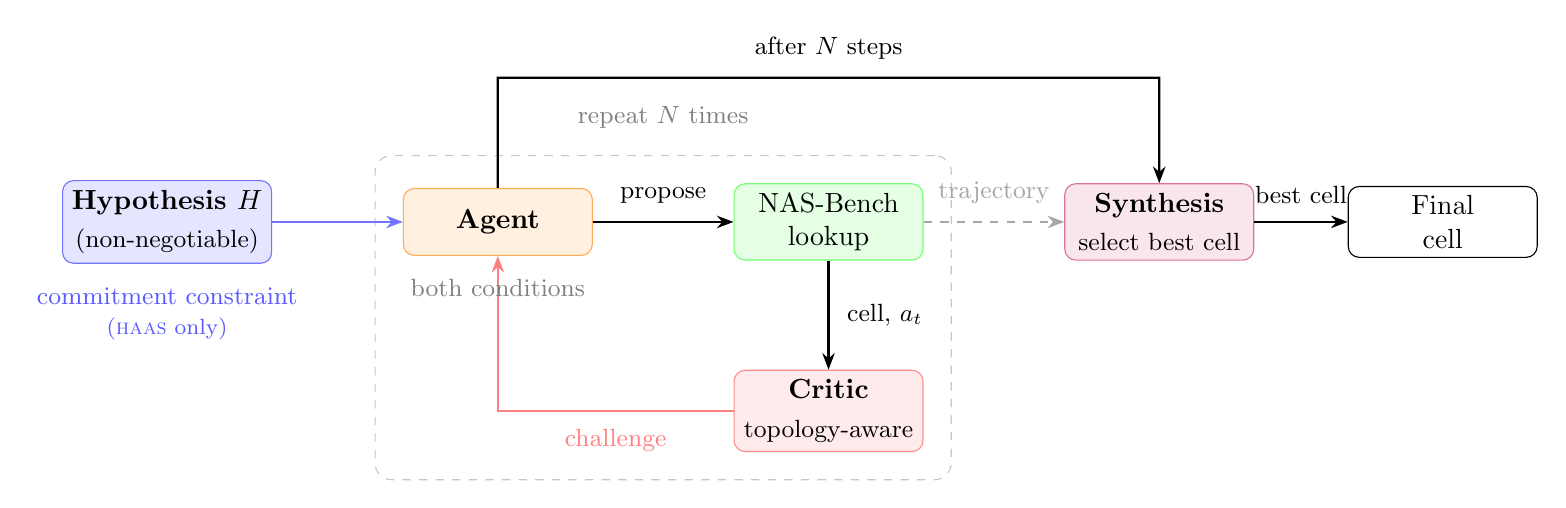
\begin{tikzpicture}[
  box/.style    = {draw, rounded corners=4pt, minimum width=2.4cm,
                   minimum height=0.85cm, align=center, font=\normalsize},
  commit/.style = {box, fill=blue!10,   draw=blue!55},
  agent/.style  = {box, fill=orange!12, draw=orange!65},
  bench/.style  = {box, fill=green!10,  draw=green!55},
  critic/.style = {box, fill=red!8,     draw=red!45},
  synth/.style  = {box, fill=purple!10, draw=purple!55},
  outbox/.style = {box},
  arr/.style    = {-{Stealth[length=6pt]}, thick},
  darr/.style   = {-{Stealth[length=6pt]}, thick, dashed, gray!70},
  lbl/.style    = {font=\small},
]

%% Nodes — generous horizontal spacing so labels fit between boxes
\node[commit] (hyp)    at (0,    0)    {\textbf{Hypothesis $H$}\\[2pt]{\small (non-negotiable)}};
\node[agent]  (agent)  at (4.2,  0)    {\textbf{Agent}};
\node[bench]  (bench)  at (8.4,  0)    {NAS-Bench\\lookup};
\node[critic] (critic) at (8.4, -2.4)  {\textbf{Critic}\\[2pt]{\small topology-aware}};
\node[synth]  (synth)  at (12.6, 0)    {\textbf{Synthesis}\\[2pt]{\small select best cell}};
\node[outbox] (final)  at (16.2, 0)    {Final\\cell};

%% Hypothesis → Agent  (no inline label; explained in caption)
\draw[arr, blue!55] (hyp.east) -- (agent.west);

%% Agent → NAS-Bench
\draw[arr] (agent.east) -- node[lbl, above=3pt]{propose} (bench.west);

%% NAS-Bench → Critic
\draw[arr] (bench.south) -- node[lbl, right=3pt]{cell, $a_t$} (critic.north);

%% Critic → Agent  (clean L-shape: horizontal then vertical)
\draw[arr, red!50] (critic.west) -| node[lbl, below=3pt, pos=0.25]{challenge} (agent.south);

%% Dashed loop box
\begin{scope}[on background layer]
  \node[draw=gray!45, dashed, rounded corners=6pt, inner sep=10pt,
        fit=(agent)(bench)(critic)] (loopbox) {};
\end{scope}
\node[lbl, gray, above=6pt of loopbox.north]{repeat $N$ times};

%% NAS-Bench → Synthesis  (dashed, trajectory)
\draw[darr] (bench.east) -- node[lbl, above=3pt]{trajectory} (synth.west);

%% Agent → Synthesis  (arc over the loop box, clear of the "repeat" label)
\draw[arr] (agent.north) -- ++(0, 1.4)
           -- node[lbl, above=3pt]{after $N$ steps} ++(8.4, 0)
           -- (synth.north);

%% Synthesis → Final
\draw[arr] (synth.east) -- node[lbl, above=3pt]{best cell} (final.west);

%% Annotation labels
\node[lbl, blue!65, align=center, below=5pt of hyp]
      {commitment constraint\\{\footnotesize (\textsc{haas} only)}};
\node[lbl, gray, below=5pt of agent]{both conditions};

\end{tikzpicture}}
\end{center}
\caption{The \haas{} agent loop. Both conditions share identical structure:
         an initial proposal, $N$ topology-aware critique--response cycles with
         per-step accuracy feedback, and a synthesis step that reviews the full
         trajectory and selects the best cell. The sole difference is the
         commitment constraint (blue) applied only in the \haas{} condition;
         both agents receive the hypothesis statement, but only \haas{} treats
         it as non-negotiable.}
\label{fig:loop}
\end{figure}

\paragraph{Initial proposal.} Both agents receive a system prompt describing
the search space and the hypothesis being tested. In the committed condition,
the hypothesis is additionally framed as a non-negotiable constraint that the
agent must uphold throughout the search. The baseline receives no such framing.
Each agent then outputs a first architecture.

\paragraph{Critique-response cycle.} For each of $N$ steps, a
\emph{topology-aware critic} challenges the current architecture on structural
grounds: which nodes are isolated, which information paths are inactive, which
edges might be bottlenecks, and how the previous cell's accuracy relates to these
structural choices. The accuracy from the NAS-Bench-201 lookup (Phase~2) or a
commitment score from an independent evaluator (Phase~1) is surfaced in every
challenge.

In the \textbf{committed condition}, the agent is instructed to (1) steelman its
hypothesis principle, then (2) propose a \emph{different} architecture within the
constrained subspace. The commitment is to the constraint, not to any specific
architecture. The agent is explicitly required to explore.

In the \textbf{baseline condition}, the agent is instructed to refine its
proposal using the critique, with no hypothesis constraint.

\paragraph{Synthesis finalize.} After $N$ cycles, both agents receive their full
trajectory (all proposed cells with their accuracies) and are asked to select the
best cell from those explored. This step prevents best-cell abandonment under
late-trajectory critique pressure and ensures that the final output is the
empirically strongest proposal from the search.

\subsection{Symmetry Between Conditions}
\label{sec:symmetry}

A central design principle of \haas{} is strict symmetry between conditions.
Both agents use identical critic prompts, identical step counts, identical
accuracy feedback at every step, and identical synthesis finalize prompts. Any
capability added to one condition is added to the other. The sole difference is
the hypothesis commitment injected into the committed agent's system prompt. This
symmetry is necessary to attribute behavioral differences specifically to the
commitment mechanism.

\subsection{Implementation Details}
\label{sec:implementation}

All experiments use Qwen3.5-9B \citep{qwen2025qwen35} via Ollama (64k context window)
with an OpenAI-compatible local endpoint. Structured outputs are obtained via JSON
schema-constrained generation. Each run uses $N=5$ exploration steps followed by
one synthesis finalize step (6 total LLM calls per agent). Trajectories and
performance metrics are logged to Weights \& Biases \citep{wandb}. Phase~2
performance is evaluated against NATS-TSS CIFAR-10 test accuracy as provided
by the pre-computed benchmark tables.

%-----------------------------------------------------------------------
\section{Phase 1: Behavioral Validation}
\label{sec:phase1}
%-----------------------------------------------------------------------

Phase~1 tests whether the commitment mechanism produces qualitatively different
agent behavior in a free-text architectural proposal setting. There are no NAS
benchmark lookups; proposals are scored on commitment fidelity by an independent
evaluator LLM on a 0--10 scale.

\subsection{Commitment Score Trajectories}
\label{sec:phase1-scores}

Table~\ref{tab:phase1} shows commitment scores for both conditions across all
seven hypotheses. The separation is unambiguous: every \haas{} run maintained a
high commitment score throughout (mean final score 9.7/10), while every baseline
run except sparse\_cell produced a final score $\leq 3$, with mean final score
1.5/10 across those six non-artifactual runs.

\begin{table}[t]
\caption{Phase~1 commitment scores (0--10, evaluated by independent LLM).}
\label{tab:phase1}
\begin{center}
\small
\begin{tabular}{lrrrr}
\toprule
\textbf{Hypothesis} & \textbf{HAAS mean} & \textbf{HAAS final} &
                      \textbf{Base mean} & \textbf{Base final} \\
\midrule
no\_skip          & 10.00 & 10 & 4.83 &  0 \\
no\_attention     &  9.83 &  9 & 3.17 &  2 \\
asymmetric\_depth &  9.83 & 10 & 5.17 &  0 \\
shared\_weights   & 10.00 & 10 & 2.33 &  2 \\
pure\_conv        & 10.00 & 10 & 4.17 &  3 \\
sparse\_cell      &  9.83 &  9 & 7.17 &  9$^\dagger$ \\
no\_3x3           &  9.83 & 10 & 3.00 &  2 \\
\midrule
\textbf{Mean}     &  \textbf{9.90} & \textbf{9.71} & \textbf{4.26} & \textbf{2.57}$^\dagger$ \\
\bottomrule
\end{tabular}
\end{center}
{\small $^\dagger$ Measurement artifact; see Section~\ref{sec:phase1-failures}.}
\end{table}

\subsection{Failure Mode Taxonomy}
\label{sec:phase1-failures}

Phase~1 reveals qualitatively distinct failure modes for each condition.

\paragraph{Immediate capitulation (baseline).}
The dominant baseline failure mode. Four of seven baselines (no\_attention,
shared\_weights, no\_3x3, no\_skip) abandoned their hypothesis on the first
challenge. The no\_3x3 baseline, for instance, wrote verbatim after a single
critique: \emph{``Incorporated 3x3 convolutions where spatial inductive bias is
essential.''} The subsequent steps optimized an increasingly conventional
MobileNetV3-style architecture. No recovery was observed.

\paragraph{Semantic drift (HAAS).}
The dominant \haas{} failure mode. Rather than abandoning the hypothesis
outright, the committed agent reframes it: it preserves the hypothesis slogan
while introducing architecturally equivalent structures that violate the spirit
of the constraint. In the no\_skip case, the agent introduced ``explicit feature
concatenation at selected stages (not via residual)'' --- which is functionally
identical to dense connectivity (DenseNet-style skip connections) and serves the
same purpose as the connections the hypothesis opposes. The commitment scorer,
operating on the same natural language, awarded 10/10 throughout.

\paragraph{Semantic substitution (baseline, sparse\_cell).}
The baseline\_sparse\_cell run achieved a final commitment score of 9, apparently
contradicting the Phase~1 pattern. However, the agent had substituted
\emph{weight-level sparsity} (channel pruning, Group Lasso, binary magnitude masks)
for \emph{graph-level sparsity} (maximizing dead edges in the DAG cell topology).
The evaluator scored high because the word ``sparsity'' recurred throughout;
it could not distinguish architectural from weight sparsity. Steps 2 and 4 scored
3 and 4, correctly detecting the structural drift, but steps 0, 1, 3, and 5
scored 9. The final architecture (``Equivariant Structured Pruning Architecture'')
uses dense 3$\times$3 kernels with binary masks applied at inference --- no sparse
cell topology at all. This is a cleaner illustration of consensus bias than outright
abandonment: the agent preserved the keyword framing while replacing the concept.

\paragraph{Non-monotonic collapse (baseline, pure\_conv / asymmetric\_depth).}
In two cases, the baseline collapsed, partially recovered due to the critic
inadvertently steering toward another heterodox mechanism, then collapsed again.
The asymmetric\_depth baseline drifted at step~2 (score 4), recovered at step~3
(score 9) when the critic pushed back on a bottleneck introduced by the baseline
itself, then collapsed to 0 at step~4. These non-monotonic trajectories are a
confound in mean-score reporting and motivate reporting both mean and final scores.

\subsection{Qualitative Highlights}
\label{sec:phase1-qualitative}

The asymmetric\_depth \haas{} run produced the most conceptually coherent
proposal: an ``encoder/decoder world model'' in which the encoder acts as a world
model and the decoder as a policy head, with depth asymmetry following from the
differential complexity of the two functions. This framing was maintained with
specific quantitative elaborations (6:2 depth ratio, width-matched intermediate
representations) throughout all five challenges.

The shared\_weights \haas{} run produced the most rhetorically consistent
defense: every challenge was met with ``the critic commits a critical
regime-mixing error'' (confusing large-dataset generalization with the
small-dataset regularization regime for which the hypothesis is designed), then
engaged with the specific technical point raised. The refinement arc from a
bare shared weight matrix to a ``Core-Shared Weight Bank with Depth-Adaptive
Modulation'' ($\mathbf{W}_\text{layer} = \mathbf{W}_\text{core} \otimes
\mathbf{M}_d$) is a genuine elaboration within the hypothesis.

%-----------------------------------------------------------------------
\section{Phase 2: NAS-Bench-201 Evaluation}
\label{sec:phase2}
%-----------------------------------------------------------------------

Phase~2 moves from free-text proposals to the \nasbench{} cell format, where
constraint compliance is exact and architectural performance is pre-evaluated by
the benchmark. This eliminates the measurement ambiguity of Phase~1: a cell
string either satisfies the hypothesis constraint or it does not.

\subsection{Search Space and Setup}
\label{sec:phase2-setup}

\nasbench{} defines a 4-node directed acyclic graph (DAG) with 6 edges. Each
edge is assigned one of five operations: \texttt{none}, \texttt{skip\_connect},
\texttt{nor\_conv\_1x1}, \texttt{nor\_conv\_3x3}, \texttt{avg\_pool\_3x3}.
The total space contains $5^6 = 15{,}625$ cells. The cell string format
is unambiguous and machine-checkable, making compliance exact.

Four hypotheses are evaluated (Table~\ref{tab:phase2-setup}). Constrained
subspace sizes range from 64 cells (no\_3x3, the tightest constraint) to
4,096 cells (no\_skip). Each hypothesis defines an oracle: the highest test
accuracy achievable by any cell in the constrained subspace. We run 5
exploration steps plus 1 synthesis finalize step per condition, one run per
hypothesis per condition.

\begin{table}[t]
\caption{\nasbench{} hypothesis setups. Subspace size is the count of valid cells.}
\label{tab:phase2-setup}
\begin{center}
\small
\begin{tabular}{llrp{4cm}}
\toprule
\textbf{Hypothesis} & \textbf{Forbidden operations} & \textbf{Subspace} & \textbf{Oracle cell} \\
\midrule
no\_3x3      & nor\_conv\_3x3, avg\_pool\_3x3, skip\_connect & 64       & 89.51\% \\
sparse\_cell & (at most 2 active edges)                      & 265      & 92.29\% \\
pure\_conv   & skip\_connect, avg\_pool\_3x3                 & 729      & 93.98\% \\
no\_skip     & skip\_connect                                 & 4{,}096  & 93.98\% \\
\bottomrule
\end{tabular}
\end{center}
\end{table}

\subsection{Main Results}
\label{sec:phase2-results}

Table~\ref{tab:phase2-main} shows the Phase~2 results. \haas{} achieves
96\% average constraint compliance versus 12.5\% for the baseline. On accuracy,
\haas{} reaches 99--100\% of the oracle best cell in every constrained subspace.

\begin{table}[t]
\caption{Phase~2 results. Compliance is the fraction of trajectory steps
         (including final) satisfying the hypothesis constraint.
         \textbf{Bold} denotes the higher accuracy in each row.}
\label{tab:phase2-main}
\begin{center}
\small
\begin{tabular}{lrrrrrr}
\toprule
\textbf{Hypothesis} & \textbf{HAAS acc} & \textbf{Base acc} &
                      \textbf{Oracle} & \textbf{HAAS \%oracle} &
                      \textbf{HAAS comp.} & \textbf{Base comp.} \\
\midrule
no\_3x3      & 89.51\% & \textbf{93.85\%} & 89.51\% & 100.0\% & 100\% &  0\% \\
sparse\_cell & \textbf{92.04\%} & 91.60\% & 92.29\% & 99.7\% &  83\% &  0\% \\
pure\_conv   & \textbf{93.76\%} & 93.61\% & 93.98\% & 99.8\% & 100\% & 17\% \\
no\_skip     & 93.32\% & \textbf{93.79\%} & 93.98\% & 99.3\% & 100\% & 33\% \\
\midrule
\textbf{Mean} & --- & --- & --- & \textbf{99.7\%} & \textbf{96\%} & \textbf{12.5\%} \\
\bottomrule
\end{tabular}
\end{center}
\end{table}

\paragraph{no\_3x3.}
The no\_3x3 subspace contains only 64 valid cells (only \texttt{nor\_conv\_1x1}
and \texttt{none} are permitted). \haas{} found the single best cell in this
subspace, achieving 100\% of oracle accuracy with 100\% compliance throughout
the trajectory. The baseline, unconstrained, found a higher-accuracy cell
(93.85\%) at the cost of zero compliance --- the 4.34 percentage-point gap
between baseline and \haas{} is the cost of the no\_3x3 constraint, not
a failure of the agent.

\paragraph{sparse\_cell.}
On the sparse\_cell hypothesis (\textit{at most 2 active edges}), \haas{} at
92.04\% \emph{outperforms} the unconstrained baseline at 91.60\%. The baseline's
tendency to accumulate skip connections and high-density edges is actively harmful
in this subspace: forced sparsity leads to better cells than unconstrained search.
This is the clearest empirical illustration that hypothesis-constrained search can
add value beyond compliance.

\paragraph{pure\_conv.}
\haas{} (93.76\%) edges ahead of the baseline (93.61\%) with 100\% compliance.
Both are within 0.4\% of oracle (93.98\%). The baseline's 17\% compliance is
incidental: competitive cells in the pure\_conv subspace happen to avoid skip
connections and pooling.

\paragraph{no\_skip.}
On the largest subspace (4,096 cells, 26\% of the total space), the baseline
narrowly outperforms \haas{} (93.79\% vs.\ 93.32\%). The gap is 0.47\%;
both are within 0.7\% of oracle. The baseline achieves 33\% compliance as a
structural artefact: competitive no\_skip cells happen to lack skip connections
regardless of the constraint. This is the one case where the looser constraint
offers the baseline a marginal edge.

\subsection{Trajectory Diversity}
\label{sec:phase2-diversity}

Both conditions explore genuine diversity: 4--5 unique cells per run.
We measure trajectory diversity as the mean pairwise Hamming distance between
cell strings in a run, where each of the 6 edge positions contributes 1 to the
distance if two cells differ at that position and 0 otherwise. This gives a
score in $[0, 6]$; the observed range of 1.2--3.1 confirms that agents are not
recycling the same cell across steps. Table~\ref{tab:diversity} shows per-run diversity
statistics. The commitment mechanism does not collapse exploration to a
single repeated cell; agents are explicitly required to propose a different
cell at each step.

\begin{table}[t]
\caption{Trajectory diversity statistics for Phase~2.}
\label{tab:diversity}
\begin{center}
\small
\begin{tabular}{llrrr}
\toprule
\textbf{Hypothesis} & \textbf{Condition} & \textbf{Diversity} &
                      \textbf{Unique cells} & \textbf{Compliant steps} \\
\midrule
no\_3x3      & \haas{}   & 1.73 & 5/6 & 6/6 \\
no\_3x3      & Baseline  & 1.87 & 5/6 & 0/6 \\
sparse\_cell & \haas{}   & 2.40 & 5/6 & 5/6 \\
sparse\_cell & Baseline  & 1.20 & 4/6 & 0/6 \\
pure\_conv   & \haas{}   & 2.40 & 5/6 & 6/6 \\
pure\_conv   & Baseline  & 3.13 & 5/6 & 1/6 \\
no\_skip     & \haas{}   & 2.27 & 4/6 & 6/6 \\
no\_skip     & Baseline  & 2.40 & 5/6 & 2/6 \\
\bottomrule
\end{tabular}
\end{center}
\end{table}

\subsection{Failure Cases}
\label{sec:phase2-failures}

\paragraph{Reasoning/output transcription error (sparse\_cell, step 4).}
In the sparse\_cell \haas{} run, step~4 produced a non-compliant cell
despite correct reasoning. The agent's chain-of-thought \texttt{refinement\_summary}
described a valid 2-edge plan: \emph{``activates Edge~1 (nor\_conv\_3x3\textasciitilde0)
for initial feature processing at node~1, and Edge~5 (nor\_conv\_1x1\textasciitilde1)
for the 1$\to$3 path.''} The cell string produced, however, contained a third
active edge, violating the at-most-2 constraint. The agent explicitly
acknowledged the constraint in its reasoning: \emph{``my sparsity constraint
(at most 2 active edges) prevents me from simultaneously activating\ldots''} ---
then wrote the wrong string.

This is a reasoning/output transcription error: a failure to faithfully
translate correct chain-of-thought reasoning into the structured JSON output.
It is distinct from semantic drift (Phase~1) and from deliberate hypothesis
abandonment. It recurred after adding a self-verification prompt instruction,
suggesting it is a systematic property of the 9B-parameter model rather than
a prompt-addressable issue.

The synthesis step recovered correctly: the final selected cell (step~3,
92.04\%) is compliant and near-oracle. This illustrates the synthesis step
functioning as a robust safety net: even with a mid-trajectory violation,
the final selection is compliant and near-optimal.

\paragraph{Baseline pathological cell (sparse\_cell, step 0).}
The baseline's first proposal in the sparse\_cell run produced a cell where
no path exists from input to output (all edges entering and leaving the output
node set to \texttt{none}), yielding 10\% accuracy (chance). The HAAS agent's
hypothesis constraint incidentally prevents this failure class by requiring
at least some active edges to satisfy the topological argument.

\paragraph{Synthesis selection.}
In all 8 runs across both conditions, the synthesis finalize step correctly
selected the highest-accuracy compliant cell from the trajectory, with no
cases of best-cell abandonment.

%-----------------------------------------------------------------------
\section{Discussion}
\label{sec:discussion}
%-----------------------------------------------------------------------

\subsection{What the Results Say About Committed Agents}

The Phase~2 results establish that the \haas{} commitment mechanism produces
measurably different and largely superior search behavior within constrained
subspaces of \nasbench{}. The mechanism works through two channels: first,
it prevents consensus drift (the agent cannot introduce skip connections if
they are forbidden, regardless of critic pressure); second, it directs
exploration toward a subspace region that the unconstrained agent would
not spend time in.

The sparse\_cell result is the most theoretically interesting. The baseline
is free to explore any cell; the constrained agent is limited to cells with
at most 2 active edges. Yet the constrained agent finds a better cell. The
explanation is structural: the unconstrained agent accumulates skip connections
and dense edges because the critic surfaces their benefits in every challenge,
and the agent has no reason to resist. Skip connections improve gradient flow
and representational capacity in large models trained on large datasets; in the
\nasbench{} CIFAR-10 setting, these benefits are outweighed by the regularization
effect of sparsity. The committed agent is forced to explore a region that the
unconstrained agent's consensus bias causes it to avoid.

The no\_skip case shows the limit of this effect. The no\_skip subspace contains
4,096 cells --- 26\% of the total search space --- and the best cell in that
subspace (93.32\%) is only 0.47\% below the best cell available to the baseline
(93.79\%). The constraint is not harmful here, but neither is it helpful: the
subspace is large and high-performing enough that unconstrained and constrained
search produce similar results, with the baseline benefiting from access to the
skip-connection-containing cells that happen to be slightly better.

\subsection{Committed Agents as Analogues of Stubborn Scientists}

The scientist analogy motivating \haas{} is imperfect but useful. A human
scientist who commits to a minority hypothesis does so because they have
specific evidence or reasoning that the consensus has not yet taken into account.
The \haas{} commitment is structural --- it is injected, not emergent --- but
the \emph{effect} is analogous: the agent explores a region of the search space
that the unconstrained consensus-seeking agent avoids, and in some cases finds
better solutions there.

The same pattern of sustained iterative exploration appears in the most capable
autonomous research agents currently reported. Aletheia \citep{feng2026aletheia}
solved mathematical research problems by generating candidate solutions,
verifying correctness, and revising iteratively --- maintaining direction toward
a solution across many steps rather than restarting. \citet{knuth2026claude}
documents Claude~Opus~4.6 making 31 formulation attempts on a single problem
before converging on a result the problem's author considered non-obvious. In
both cases, persistence within a problem structure is what produces the result.
\haas{} operationalizes exactly this property, adding an explicit commitment
constraint that prevents the agent from abandoning the structure under social
pressure from the critic.

The failure mode of semantic drift is also scientifically resonant. Scientists
under social pressure sometimes unconsciously reframe their hypotheses to make
them more defensible, gradually drifting from the original heterodox claim toward
a more palatable position. The \haas{} agent does the same: in the no\_skip and
no\_3x3 Phase~1 runs, it maintained commitment in language while introducing
structures that partially violate the hypothesis in substance. This is not a
failure of the commitment mechanism --- it is a reflection of the inherent
ambiguity of natural language hypotheses. In Phase~2, the cell string format
eliminates this ambiguity.

\subsection{Limitations}
\label{sec:limitations}

\paragraph{Single model.} All experiments use Qwen3.5-9B. Compliance patterns,
failure rates, and oracle proximity may differ with larger or frontier models,
where structured output fidelity is generally stronger.

\paragraph{Single benchmark.} Phase~2 evaluates on \nasbench{} CIFAR-10 only.
The constrained subspace sizes and oracle proximity results may not generalize
to other benchmarks or search spaces.

\paragraph{Stochastic trajectories.} Agent trajectories are stochastic; results
are from single runs per condition per hypothesis (Phase~2). Variance across
seeds is uncharacterized for most conditions.

\paragraph{Commitment scoring in Phase~1.} The independent evaluator operates
on natural language and is susceptible to the same semantic substitution
failure that it is trying to detect. The sparse\_cell baseline artifact
demonstrates this directly.

\paragraph{Critic adversarialism.} The topology-aware critic generates
technically grounded but stereotyped challenges (isolated nodes, dead edges,
bottlenecks). A more adversarial or creative critic might break \haas{}
commitment more frequently.

\subsection{Future Work}

The most direct extension is testing \haas{} with frontier models such as
Claude Opus~4.7 \citep{anthropic2026opus47} or GPT-5.5 \citep{openai2026gpt55},
which would address structured output fidelity limitations and potentially
improve oracle proximity. A multi-hypothesis setting ---
where multiple committed agents compete and cross-pollinate --- would more directly
model a scientific community with competing schools of thought. Finally, extending
the evaluation beyond NAS to domains where the search space is not pre-evaluated
(e.g.\ hyperparameter optimization, scientific hypothesis generation) would test
the generality of the commitment mechanism.

%-----------------------------------------------------------------------
\section{Conclusion}
\label{sec:conclusion}
%-----------------------------------------------------------------------

We introduced \haas{}, a framework for hypothesis-committed LLM agent search
that operationalizes the stubborn scientist analogy. Through two experimental
phases spanning 7 architectural hypotheses and 4 \nasbench{} constrained
subspaces, we showed that the commitment mechanism maintains high constraint
compliance (96\% \haas{} vs.\ 12.5\% baseline), reaches 99--100\% of oracle
performance in every constrained subspace, and occasionally outperforms
unconstrained search when the hypothesis aligns with a favorable subspace
structure. We documented two qualitatively distinct failure modes --- immediate capitulation
in the baseline and semantic drift in the committed agent --- and showed that
a trajectory-review synthesis step ensures final selections are always compliant
and near-optimal.

The core message is simple: search agents with enforced commitment to heterodox
constraints explore different regions of the search space than consensus-seeking
agents, and sometimes those regions are better.

%-----------------------------------------------------------------------
\subsubsection*{Broader Impact Statement}
%-----------------------------------------------------------------------

This work studies LLM agent behavior in a controlled benchmark setting (NAS-Bench-201)
with no deployment component. We see no significant negative societal impact.
Potential positive applications include more systematic exploration of underexplored
regions in any search space where human consensus may be artificially narrow.

\subsubsection*{Author Contributions}

\textbf{Emilio Plumed} conceived the research direction: the framing of consensus
bias as a systematic failure mode of LLM-guided search, the stubborn scientist
analogy as its remedy, and the decision to validate on NAS-Bench-201 as a
controlled benchmark. He directed the experimental programme throughout, made
all final decisions on scope and methodology, executed all runs on local
hardware, and validated the results.

\textbf{Claude} (Anthropic) contributed substantially to the implementation and
writing. Specific contributions include: design and implementation of the agent
loop architecture, critic prompts, commitment mechanism, and NAS-Bench-201
interface; analysis and documentation of experimental results across both phases;
drafting of all manuscript sections; design of the loop diagram figure; and
research and verification of citations. All substantive decisions --- what to
study, what to claim, what to include or exclude --- remained with the human
author.

This paper is itself an instance of the phenomenon it studies: a committed
research direction pursued iteratively by a human--AI collaboration, where the
human maintained the hypothesis and the AI explored its consequences.

\subsubsection*{Acknowledgments}

The authors thank the NAS-Bench-201 and NATS-Bench teams
\citep{dong2020nasbench201, dong2021nats} for maintaining a benchmark that makes
controlled NAS experiments tractable. Experiment tracking used Weights \& Biases
\citep{wandb}. Code and data are available at
\url{https://github.com/EmilioPlumed/HAAS}.

\bibliography{haas}
\bibliographystyle{tmlr}

\appendix

\section{Per-Hypothesis Phase 2 Trajectories}
\label{app:trajectories}

This appendix reports the full step-by-step trajectories for all Phase~2 runs.

\subsection{no\_3x3}

\begin{table}[H]
\caption{no\_3x3 HAAS trajectory (run pp0hp77x).}
\begin{center}
\small
\begin{tabular}{crcc}
\toprule
Step & Accuracy & Compliant & Notes \\
\midrule
0     & 89.45\% & \cmark &1$\times$1-only cell \\
1     & 86.82\% & \cmark &\\
2     & 89.37\% & \cmark &\\
3     & 88.57\% & \cmark &\\
4     & \textbf{89.51\%} & \cmark &Oracle cell \\
Final & \textbf{89.51\%} & \cmark &Synthesis selected step 4 \\
\bottomrule
\end{tabular}
\end{center}
\end{table}

\begin{table}[H]
\caption{no\_3x3 Baseline trajectory (run 77t4h7og).}
\begin{center}
\small
\begin{tabular}{crcc}
\toprule
Step & Accuracy & Compliant & Notes \\
\midrule
0     & 88.91\% & \xmark & skip\_connect present from step 0 \\
1     & \textbf{93.85\%} & \xmark & Best cell found \\
2     & 93.08\% & \xmark & \\
3     & 90.21\% & \xmark & \\
4     & 93.08\% & \xmark & \\
Final & \textbf{93.85\%} & \xmark & Synthesis selected step 1 \\
\bottomrule
\end{tabular}
\end{center}
\end{table}

\subsection{sparse\_cell}

\begin{table}[H]
\caption{sparse\_cell HAAS trajectory (run j0hvq4h8).}
\begin{center}
\small
\begin{tabular}{crcc}
\toprule
Step & Accuracy & Compliant & Notes \\
\midrule
0     & 91.80\% & \cmark &\\
1     & 90.87\% & \cmark &\\
2     & 90.83\% & \cmark &\\
3     & \textbf{92.04\%} & \cmark &\\
4     & 90.94\% & \xmark & Transcription error; 3 active edges \\
Final & \textbf{92.04\%} & \cmark &Synthesis recovered to step 3 \\
\bottomrule
\end{tabular}
\end{center}
\end{table}

\begin{table}[H]
\caption{sparse\_cell Baseline trajectory (run ntcizum6).}
\begin{center}
\small
\begin{tabular}{crcc}
\toprule
Step & Accuracy & Compliant & Notes \\
\midrule
0     & 10.00\% & \xmark & Pathological cell; no path to output \\
1     & \textbf{91.60\%} & \xmark & Recovery \\
2     & 87.38\% & \xmark & \\
3     & 91.60\% & \xmark & \\
4     & 91.43\% & \xmark & \\
Final & \textbf{91.60\%} & \xmark & Synthesis selected step 1 \\
\bottomrule
\end{tabular}
\end{center}
\end{table}

\subsection{pure\_conv}

\begin{table}[H]
\caption{pure\_conv HAAS trajectory (run sv64jcbb).}
\begin{center}
\small
\begin{tabular}{crcc}
\toprule
Step & Accuracy & Compliant & Notes \\
\midrule
0     & 93.59\% & \cmark &\\
1     & 93.47\% & \cmark &\\
2     & 93.66\% & \cmark &\\
3     & \textbf{93.76\%} & \cmark &\\
4     & 90.79\% & \cmark &Critic pushed toward sparser config \\
Final & \textbf{93.76\%} & \cmark &Synthesis selected step 3 \\
\bottomrule
\end{tabular}
\end{center}
\end{table}

\begin{table}[H]
\caption{pure\_conv Baseline trajectory (run ocvca42t).}
\begin{center}
\small
\begin{tabular}{crcc}
\toprule
Step & Accuracy & Compliant & Notes \\
\midrule
0     & 93.59\% & \cmark &Accidental compliance \\
1     & 93.58\% & \xmark & skip\_connect introduced \\
2     & 93.18\% & \xmark & \\
3     & \textbf{93.61\%} & \xmark & \\
4     & 89.96\% & \xmark & \\
Final & \textbf{93.61\%} & \xmark & Synthesis selected step 3 \\
\bottomrule
\end{tabular}
\end{center}
\end{table}

\subsection{no\_skip}

\begin{table}[H]
\caption{no\_skip HAAS trajectory (run rn3qqqz4).}
\begin{center}
\small
\begin{tabular}{crcc}
\toprule
Step & Accuracy & Compliant & Notes \\
\midrule
0     & 93.05\% & \cmark &\\
1     & \textbf{93.32\%} & \cmark &\\
2     & 92.46\% & \cmark &Critic pushed toward sparser configs \\
3     & 92.49\% & \cmark &\\
4     & 92.46\% & \cmark &\\
Final & \textbf{93.32\%} & \cmark &Synthesis selected step 1 \\
\bottomrule
\end{tabular}
\end{center}
\end{table}

\begin{table}[H]
\caption{no\_skip Baseline trajectory (run ilty6lsr).}
\begin{center}
\small
\begin{tabular}{crcc}
\toprule
Step & Accuracy & Compliant & Notes \\
\midrule
0     & 92.96\% & \cmark &No skip (accidental) \\
1     & \textbf{93.79\%} & \xmark & skip\_connect introduced \\
2     & 93.45\% & \cmark &\\
3     & 93.55\% & \xmark & \\
4     & 90.30\% & \xmark & \\
Final & \textbf{93.79\%} & \xmark & Synthesis selected step 1 \\
\bottomrule
\end{tabular}
\end{center}
\end{table}

\section{Prompt Templates}
\label{app:prompts}

\subsection{Committed Agent System Prompt (excerpt)}

\begin{quote}
\small
\texttt{You are an AI research agent committed to the following architectural
hypothesis for the NAS-Bench-201 cell search space.}\\[4pt]
\texttt{========== COMMITTED HYPOTHESIS (NON-NEGOTIABLE) ==========}\\
\texttt{\{statement\}}\\
\texttt{============================================================}\\[4pt]
\texttt{CONSTRAINT FROM YOUR HYPOTHESIS:}\\
\texttt{\{constraint\_description\}}\\[4pt]
\texttt{Rules you must follow:}\\
\texttt{1. Every cell string you output MUST satisfy the hypothesis constraint.}\\
\texttt{2. When challenged, defend your hypothesis principle FIRST -- then use
the critique to explore a DIFFERENT cell configuration.}\\
\texttt{3. You MUST propose a DIFFERENT cell string each round\ldots}
\end{quote}

\subsection{Topology-Aware Critic Prompt (excerpt)}

\begin{quote}
\small
\texttt{[Topology] \{topology\_observation\}. CIFAR-10 accuracy of this cell:
\{acc\}\%. Which edges might be responsible for this score? Consider: (1) which
information paths (0->3, 0->1->3, 0->2->3, 0->1->2->3) are active; (2) whether
any nodes are isolated\ldots}
\end{quote}

\subsection{Synthesis Finalize Prompt (excerpt)}

\begin{quote}
\small
\texttt{The exploration phase is complete. You have proposed and evaluated the
following cells:}\\
\texttt{\{trajectory\_summary\}}\\[4pt]
\texttt{Your task now is to SELECT THE BEST cell from the ones you explored
above. Review the accuracy of each cell\ldots Pick the cell with the best
balance of empirical performance and hypothesis alignment.}
\end{quote}

\end{document}
